\documentclass[tikz,convert={outfile=\jobname.svg}]{standalone}
\usetikzlibrary{patterns}
\begin{document}
    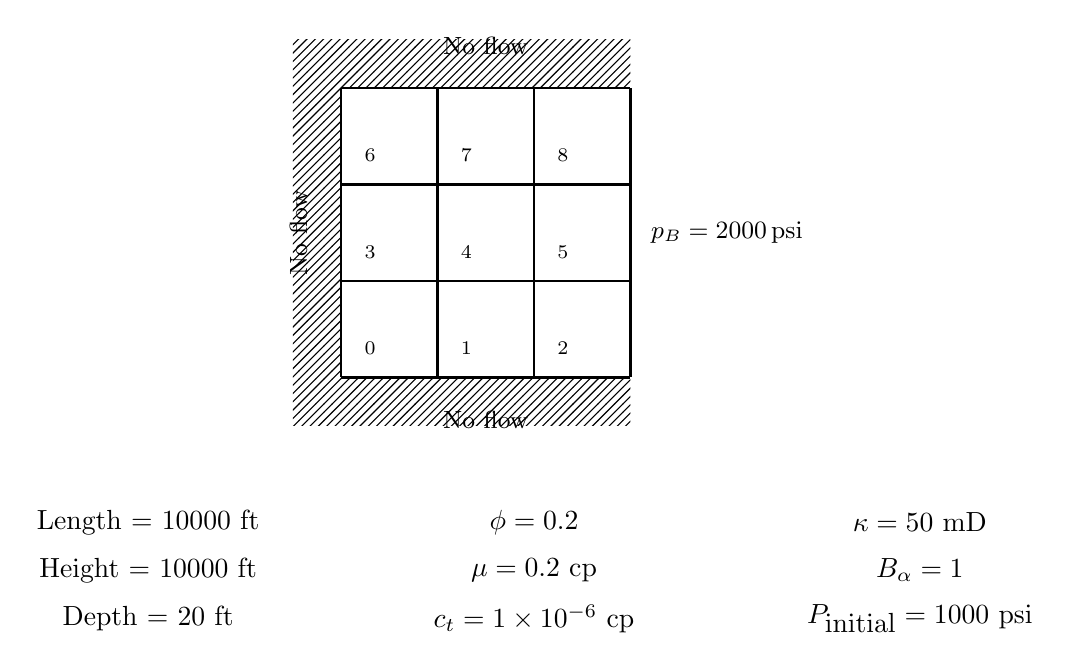
\begin{tikzpicture}[scale=2.45]
    %\foreach \i in {\xMin,...,\xMax} {
        %\draw [very thin,gray,dashed] (\i,\yMin) -- (\i,\yMax)  node [below] at (\i,\yMin) {};
    %}
    %\foreach \i in {\yMin,...,\yMax} {
        %\draw [very thin,gray,dashed] (\xMin,\i) -- (\xMax,\i) node [left] at (\xMin,\i) {};
    %}
    %\foreach \i in {7.5,8.0,8.5,9.0,9.5} {
        %\draw [very thin,gray,dashed] (\i,3.5) -- (\i,5.5)  node [below] at (\i,\yMin) {};
    %}
    %\foreach \i in {3.5,4.0,4.5,5.0,5.5} {
        %\draw [very thin,gray,dashed] (7.5,\i) -- (9.5,\i) node [left] at (\xMin,\i) {};
    %}
    \node[font=\scriptsize] at (7.65, 3.65) {0};
    \node[font=\scriptsize] at (8.15, 3.65) {1};
    \node[font=\scriptsize] at (8.65, 3.65) {2};
    \node[font=\scriptsize] at (7.65, 4.15) {3};
    \node[font=\scriptsize] at (8.15, 4.15) {4};
    \node[font=\scriptsize] at (8.65, 4.15) {5};
    \node[font=\scriptsize] at (7.65, 4.65) {6};
    \node[font=\scriptsize] at (8.15, 4.65) {7};
    \node[font=\scriptsize] at (8.65, 4.65) {8};
    \draw [thick] (7.5,3.5) -- (9.,3.5);
    \draw [thick] (7.5,4.0) -- (9.,4.0);
    \draw [thick] (7.5,4.5) -- (9.,4.5);
    \draw [thick] (7.5,3.5) -- (7.5,5);
    \draw [thick] (7.5,5) -- (9.,5);
    \draw [thick] (8.0,3.5) -- (8.0,5);
    \draw [thick] (8.5,3.5) -- (8.5,5);
    \draw [thick] (9.0,3.5) -- (9.0,5);
    \fill [pattern=north east lines] (7.5,3.25) rectangle (9.0,3.5) node [below, midway, font=\small] {No flow};
    \fill [pattern=north east lines] (7.25,3.25) rectangle (7.5,5.25) node [above, rotate=90, font=\small, midway] {No flow};
    \fill [pattern=north east lines] (7.5,5.0) rectangle (9.0,5.25) node [above, font=\small, midway] {No flow};
    \node[font=\small] at (9.5,4.25) {$p_B = 2000\,$psi};
    \node[] at (6.5, 2.75) {Length = $10000$ ft};
    \node[] at (6.5, 2.5) {Height = $10000$ ft};
    \node[] at (6.5, 2.25) {Depth = $20$ ft};
    \node[] at (8.5, 2.75) {$\phi = 0.2$};
    \node[] at (8.5, 2.5) {$\mu = 0.2$ cp};
    \node[] at (8.5, 2.25) {$c_t = 1 \times 10^{-6}$ cp};
    \node[] at (10.5, 2.75) {$\kappa = 50$ mD};
    \node[] at (10.5, 2.5) {$B_\alpha = 1$};
    \node[] at (10.5, 2.25) {$P_{\mbox{initial}} = 1000$ psi};
\end{tikzpicture}
\end{document}
